\section{Validation of the NEMO-Pisces model}
\label{sec:pisces}

The ocean fish biomass is strongly influenced by the physical and geochemical state of the ocean. Therefore, it is important to determine whether the NEMO-Pisces model, which is used to force the Apecosm model, reproduces the expected response to ENSO variability. The aim of the present section is to compare the sea-surface temperature and chlorophyll simulated by the model with observation based datasets.

\subsection{Ocean Nino Index and \sst\ signature}
\label{sec:sst}

As a first step, the Ocean Nino Index (ONI\footnote{\url{https://www.cpc.ncep.noaa.gov/data/indices/oni.ascii.txt}}) has been compared with the simulated one, in order to determine whether the timing of simulated ENSO events is consistent with the observed one. The correlation coefficient between the two monthly time-series over the overlapping period (1958-2018) is $0.94$, which gives confidence in the model ability to reproduce the observed ENSO variability. \\

In order to infer the spatial \sst\ pattern associated with the ONI index, covariance between the ONI index and the NEMO-Pisces \sst\ has been computed. Since the main focus is on the interannual variability, the covariances are applied on yearly time series. The ONI index has been averaged over boreal winter (from November to January), when most of the ENSO variability occurs. In order to insure continuity over the winter months, when ENSO variability usually peaks, yearly means of physical and biogeochemical variables have been computed from May (year $y$) to April (year $y + 1$), as done in \cite{racaultImpactNinoVariability2017}. Then, the obtained time-series has been detrended.\\

The correlation between the ONI index and the sea-surface temperature is shown in figure \ref{fig:cov-sst}. For comparison, the same analysis has been performed with the Hadley SST dataset \citep{raynerGlobalAnalysesSea2003}.
The covariance patterns are very similar between Hadley and simulated SST, with warm anomalies (1\degree C) centerred at the equator and extending from 0 to 90\degree E and from 10\degree S to 10N.\ 
The covariance along the equatorial temperature section (not shown) shows that the maximum temperature anomalies is at around 50m depth at a longitude of 70\degree E. Negative anomalies (-0.8\degree C) are located on the western part of the basin (20\degree W). This dipolar structure is consistent with a shoaling of the thermocline in the west and a deepening in the east.\\

\begin{figure}[h!]
	\centering
	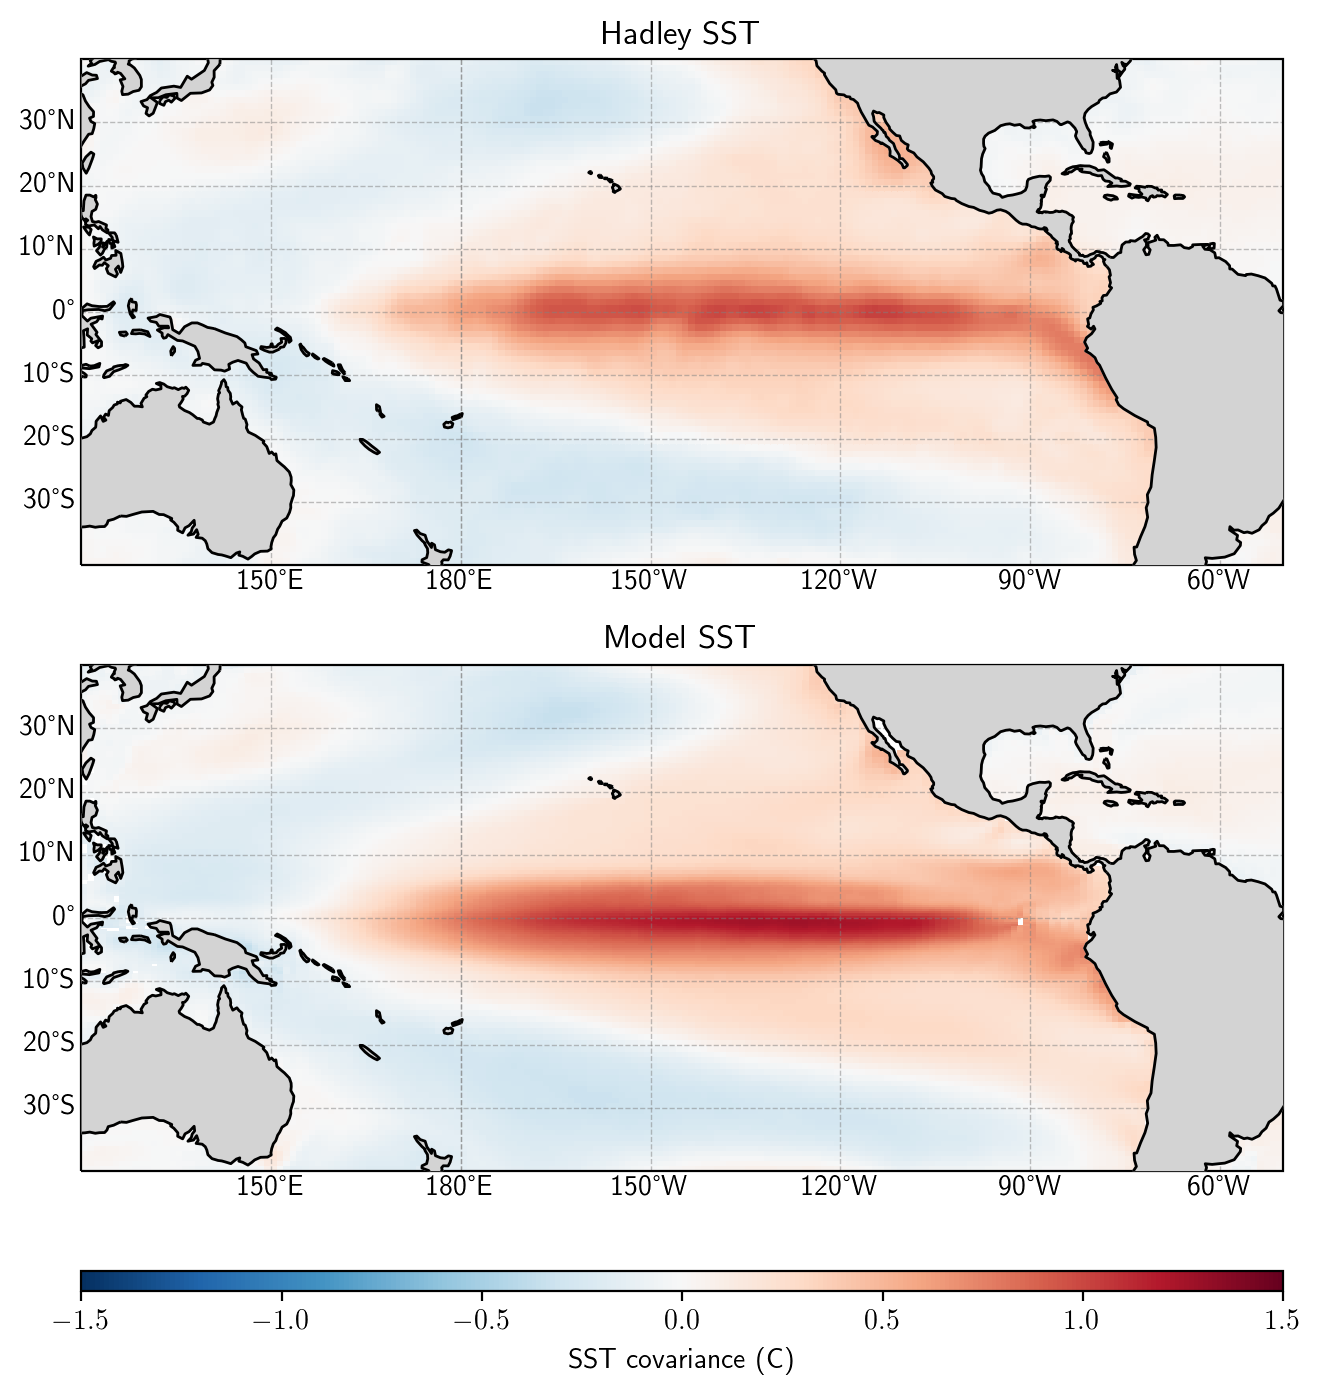
\includegraphics[scale=0.75] {scripts/cov-hadley/covariance_maps_hadley_model.png}
	\caption{Covariance between winter ONI index and Hadley (top) and simulated (bottom) yearly SST anomalies.}
	\label{fig:cov-sst}
\end{figure}

\subsection{Observed and simulated sea-surface chlorophyll}

In order to validate the biogeochemical response of the NEMO-Pisces model, satellite based observations of ocean colour \citep{sathyendranathOceanColourTimeSeries2019} have been used. The OceanColour-CCI V5 dataset provides monthly chlorophyl-a with a horizontal resolution of $1/24$\degree . First, data were Pacific-centerred and regridded to a one degree resolution. This was done by computing the weighted mean over $24 \times 24$ boxes, the weights being provided by the cosine of latitude. Coarse resolution grid cells that contained more than $1/3$ of missing data were considered as missing. Then, a monthly climatology was computed over the 1998-2020 period and removed from the observations. Finally, the covariance between these monthly anomalies and the monthly ONI index was computed between 1997-09 and 2018-12.  In a similar way, the covariance between the ONI index and the simulated surface chlorophyll was computed over the same period.\\

Covariance maps between the surface chlorophyll and the monthly ONI index are shown in figure \ref{fig:chl-cov}. The observations (upper panel) and the model (lower panel) show very similar covariance pattern, with a decrease in chlorophyll concentration in the tropical Pacific ocean, which is consistent with a reduction of the equatorial upwelling induced by the reduction and eventually reversal of the trade winds (\warn{REF}). However, the model overestimates the chlorophyll response to ENSO variability compared with observational based estimates. Note that the covariance for the simulated chlorophyll has also been computed over the entire simulated period (1958-2018), with no significant changes in the resulting pattern (not shown). \\

\begin{figure}[h!]
	\centering
	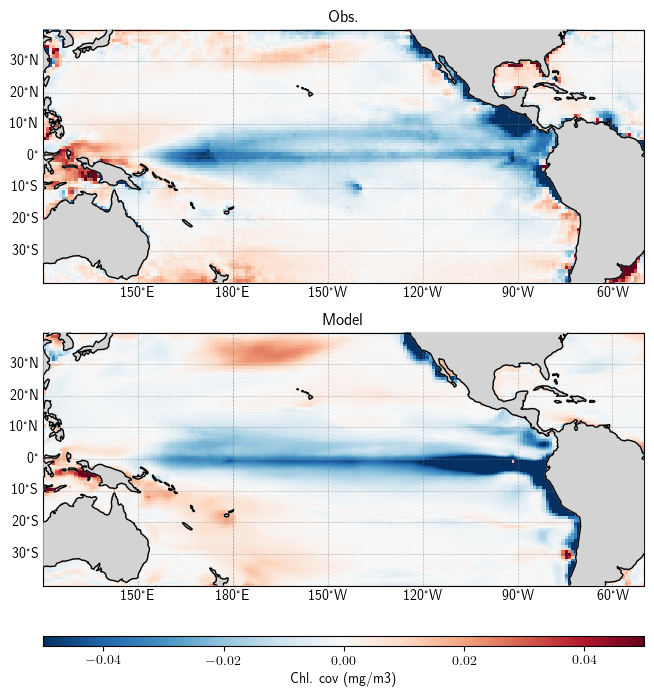
\includegraphics[scale=0.75] {scripts/chl-sat/compare_covariance_chl.png}
	\caption{Covariance between the monthly ONI index and the monthly surface chlorophyll anomalies, computed between 1997-09 and 20018-12.}
	\label{fig:chl-cov}
\end{figure}